\documentclass[]{article}
\usepackage{lmodern}
\usepackage{amssymb,amsmath}
\usepackage{ifxetex,ifluatex}
\usepackage{fixltx2e} % provides \textsubscript
\ifnum 0\ifxetex 1\fi\ifluatex 1\fi=0 % if pdftex
  \usepackage[T1]{fontenc}
  \usepackage[utf8]{inputenc}
\else % if luatex or xelatex
  \ifxetex
    \usepackage{mathspec}
  \else
    \usepackage{fontspec}
  \fi
  \defaultfontfeatures{Ligatures=TeX,Scale=MatchLowercase}
\fi
% use upquote if available, for straight quotes in verbatim environments
\IfFileExists{upquote.sty}{\usepackage{upquote}}{}
% use microtype if available
\IfFileExists{microtype.sty}{%
\usepackage{microtype}
\UseMicrotypeSet[protrusion]{basicmath} % disable protrusion for tt fonts
}{}
\usepackage[margin=1in]{geometry}
\usepackage{hyperref}
\hypersetup{unicode=true,
            pdftitle={DSCI 522 Analysis of PM 2.5 in Beijing and Shanghai},
            pdfauthor={Ting Pan, Weishun Deng},
            pdfborder={0 0 0},
            breaklinks=true}
\urlstyle{same}  % don't use monospace font for urls
\usepackage{longtable,booktabs}
\usepackage{graphicx,grffile}
\makeatletter
\def\maxwidth{\ifdim\Gin@nat@width>\linewidth\linewidth\else\Gin@nat@width\fi}
\def\maxheight{\ifdim\Gin@nat@height>\textheight\textheight\else\Gin@nat@height\fi}
\makeatother
% Scale images if necessary, so that they will not overflow the page
% margins by default, and it is still possible to overwrite the defaults
% using explicit options in \includegraphics[width, height, ...]{}
\setkeys{Gin}{width=\maxwidth,height=\maxheight,keepaspectratio}
\IfFileExists{parskip.sty}{%
\usepackage{parskip}
}{% else
\setlength{\parindent}{0pt}
\setlength{\parskip}{6pt plus 2pt minus 1pt}
}
\setlength{\emergencystretch}{3em}  % prevent overfull lines
\providecommand{\tightlist}{%
  \setlength{\itemsep}{0pt}\setlength{\parskip}{0pt}}
\setcounter{secnumdepth}{0}
% Redefines (sub)paragraphs to behave more like sections
\ifx\paragraph\undefined\else
\let\oldparagraph\paragraph
\renewcommand{\paragraph}[1]{\oldparagraph{#1}\mbox{}}
\fi
\ifx\subparagraph\undefined\else
\let\oldsubparagraph\subparagraph
\renewcommand{\subparagraph}[1]{\oldsubparagraph{#1}\mbox{}}
\fi

%%% Use protect on footnotes to avoid problems with footnotes in titles
\let\rmarkdownfootnote\footnote%
\def\footnote{\protect\rmarkdownfootnote}

%%% Change title format to be more compact
\usepackage{titling}

% Create subtitle command for use in maketitle
\newcommand{\subtitle}[1]{
  \posttitle{
    \begin{center}\large#1\end{center}
    }
}

\setlength{\droptitle}{-2em}

  \title{DSCI 522 Analysis of PM 2.5 in Beijing and Shanghai}
    \pretitle{\vspace{\droptitle}\centering\huge}
  \posttitle{\par}
    \author{Ting Pan, Weishun Deng}
    \preauthor{\centering\large\emph}
  \postauthor{\par}
      \predate{\centering\large\emph}
  \postdate{\par}
    \date{November 22, 2018}


\begin{document}
\maketitle

\section{Report}\label{report}

\subsection{Introduction}\label{introduction}

This project is to conduct research on the inferential question -
\textbf{Is the average PM2.5 in Beijing same as that in Shanghai?} We
want to explore whether the average PM2.5 in Beijing is different from
that in Shanghai in general. The datasets we choose are
\href{https://www.kaggle.com/uciml/pm25-data-for-five-chinese-cities}{PM2.5
Data of Five Chinese Cities from Kaggle.com}, which record PM2.5 of five
Chinese cities during 2010 to 2015. Because we only care about PM2.5 in
Beijing and Shanghai, these two raw datasets are as below:

\emph{Table 1. Beijing PM2.5 Raw Dataset}

\begin{longtable}[]{@{}rrrrrrrrrrrrrrlrrr@{}}
\toprule
No & year & month & day & hour & season & PM\_Dongsi & PM\_Dongsihuan &
PM\_Nongzhanguan & PM\_US.Post & DEWP & HUMI & PRES & TEMP & cbwd & Iws
& precipitation & Iprec\tabularnewline
\midrule
\endhead
1 & 2010 & 1 & 1 & 0 & 4 & NA & NA & NA & NA & -21 & 43 & 1021 & -11 &
NW & 1.79 & 0 & 0\tabularnewline
2 & 2010 & 1 & 1 & 1 & 4 & NA & NA & NA & NA & -21 & 47 & 1020 & -12 &
NW & 4.92 & 0 & 0\tabularnewline
3 & 2010 & 1 & 1 & 2 & 4 & NA & NA & NA & NA & -21 & 43 & 1019 & -11 &
NW & 6.71 & 0 & 0\tabularnewline
4 & 2010 & 1 & 1 & 3 & 4 & NA & NA & NA & NA & -21 & 55 & 1019 & -14 &
NW & 9.84 & 0 & 0\tabularnewline
5 & 2010 & 1 & 1 & 4 & 4 & NA & NA & NA & NA & -20 & 51 & 1018 & -12 &
NW & 12.97 & 0 & 0\tabularnewline
6 & 2010 & 1 & 1 & 5 & 4 & NA & NA & NA & NA & -19 & 47 & 1017 & -10 &
NW & 16.10 & 0 & 0\tabularnewline
\bottomrule
\end{longtable}

\emph{Table 2. Shanghai PM2.5 Raw Dataset}

\begin{longtable}[]{@{}rrrrrrrrrrrrrlrrr@{}}
\toprule
No & year & month & day & hour & season & PM\_Jingan & PM\_US.Post &
PM\_Xuhui & DEWP & HUMI & PRES & TEMP & cbwd & Iws & precipitation &
Iprec\tabularnewline
\midrule
\endhead
1 & 2010 & 1 & 1 & 0 & 4 & NA & NA & NA & -6 & 59.48 & 1026.1 & 1 & cv &
1 & 0 & 0\tabularnewline
2 & 2010 & 1 & 1 & 1 & 4 & NA & NA & NA & -6 & 59.48 & 1025.1 & 1 & SE &
2 & 0 & 0\tabularnewline
3 & 2010 & 1 & 1 & 2 & 4 & NA & NA & NA & -7 & 59.21 & 1025.1 & 0 & SE &
4 & 0 & 0\tabularnewline
4 & 2010 & 1 & 1 & 3 & 4 & NA & NA & NA & -6 & 63.94 & 1024.0 & 0 & SE &
5 & 0 & 0\tabularnewline
5 & 2010 & 1 & 1 & 4 & 4 & NA & NA & NA & -6 & 63.94 & 1023.0 & 0 & SE &
8 & 0 & 0\tabularnewline
6 & 2010 & 1 & 1 & 5 & 4 & NA & NA & NA & -7 & 59.21 & 1023.0 & 0 & SE &
11 & 0 & 0\tabularnewline
\bottomrule
\end{longtable}

To analyze the data efficiently, we need to do data wrangling on
\texttt{Table\ 1} and \texttt{Table\ 2}:

\begin{itemize}
\item
  For each table, add a column \texttt{PM\_Average} to record the
  average PM2.5.
\item
  For each table, add a column \texttt{city} to indicate this
  categorical variable.
\item
  Combine the two tables into one, which is \texttt{Table\ 3}.
\end{itemize}

\emph{Table 3. Beijing and Shanghai PM2.5 Tidy Dataset}

\begin{longtable}[]{@{}rrrrl@{}}
\toprule
year & month & day & PM\_Average & city\tabularnewline
\midrule
\endhead
2010 & 1 & 1 & 129.0000 & Beijing\tabularnewline
2010 & 1 & 1 & NA & Shanghai\tabularnewline
2010 & 1 & 2 & 144.3333 & Beijing\tabularnewline
2010 & 1 & 2 & NA & Shanghai\tabularnewline
2010 & 1 & 3 & 78.3750 & Beijing\tabularnewline
2010 & 1 & 3 & NA & Shanghai\tabularnewline
\bottomrule
\end{longtable}

\subsection{Visualization}\label{visualization}

To understand the tidy dataset, we take two plots to visualize it.

\subsubsection{Histogram}\label{histogram}

\emph{Figure 1. Histograms of Beijing PM2.5 and Shanghai PM2.5}

\begin{figure}
\centering
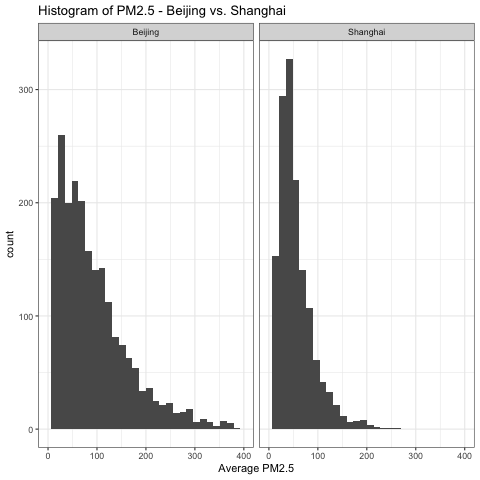
\includegraphics{../results/histogram.png}
\caption{}
\end{figure}

It shows the distributions of PM2.5 in Shanghai and Beijing. Both are
right-skewed. Looking at the distribution of Beijing, the peak occurs at
25, and the data spread is from about 0 to 400. In contrast, the peak in
distribution of Shanghai occurs at 50, which is larger than that of
Beijing. The data spread of Shanghai is from 0 to 250, which is much
narrower.

\subsubsection{Boxplot}\label{boxplot}

\emph{Figure 2. Boxplots of Beijing PM and Shanghai PM}

\begin{figure}
\centering
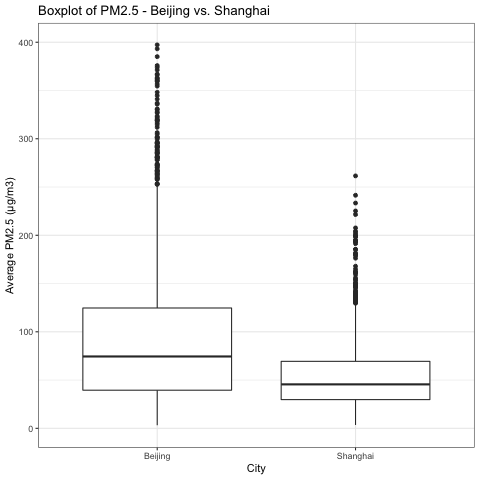
\includegraphics{../results/boxplot.png}
\caption{}
\end{figure}

It helps analyze the relationship between the categorical variable
\texttt{city} and the continuous variable \texttt{PM\_Average}. We
observe that the median PM2.5 of Beijing is higher than that of Beijing.
Also, the boxplot of Shanghai is comparatively short, which suggests
that overall PM2.5 values of Shanghai are denser. In addition, they both
have much outliers, which reveals that there are a lot of ralatively
high PM2.5 values detected in both cities.

\subsection{Data Summary}\label{data-summary}

For each city, we can easily get the sample size, the sample mean, and
the standard deviation of the sample mean. Then, assuming statistical
independence of the two groups, the standard error of the mean of each
city can be estimated as the sample standard deviation divided by the
square root of the sample size \texttt{SE\ =\ s\ /\ sqrt(n)}.
Additionally, we calculate 95\% confidence interval of PM2.5 for each
city using asymoptotic theory:
\texttt{Confidence\ Interval\ =\ (mean\ -\ \ 1.96\ *\ SE,\ mean\ +\ \ 1.96\ *\ SE)}.

\emph{Table 4. Summarize Beijing and Shanghai PM2.5 Tidy Dataset}

\begin{longtable}[]{@{}lrrrrr@{}}
\toprule
city & n & mean\_PM & se\_PM & lower\_ci & upper\_ci\tabularnewline
\midrule
\endhead
Beijing & 2155 & 95.21643 & 1.6473701 & 91.98765 &
98.44522\tabularnewline
Shanghai & 1460 & 54.81167 & 0.9888218 & 52.87362 &
56.74973\tabularnewline
\bottomrule
\end{longtable}

From \texttt{Table\ 4}, we find that the PM2.5 means of Beijing and
Shanghai are totally different. Also, we are 95\% confident that the
average PM2.5 in Beijing is between 91.98765 and 98.44522.
Comparatively, we are 95\% confident that the average PM2.5 in Shanghai
is between 52.87362 and 56.74973.

\subsection{Analysis and results}\label{analysis-and-results}

We performed the Welch's two sample t-test intead of student t-test in
this case. The main reason is that we have a lot of missing data in both
of our datasets and the sizes of two samples are different so the
homogeneous assumption of student t-test may not be hold. Another reason
is that when we perform Welch's t-test we will not pool the sample
standard deviations and this could give us a more accurate result.

The following is our test result:

\emph{Table 5. Summarize Beijing and Shanghai PM2.5 Tidy Dataset}

\begin{longtable}[]{@{}rrrrrrrrll@{}}
\toprule
estimate & estimate1 & estimate2 & statistic & p.value & parameter &
conf.low & conf.high & method & alternative\tabularnewline
\midrule
\endhead
40.40476 & 95.21643 & 54.81167 & 21.02933 & 2.597003e-92 & 3344.741 &
36.63762 & 44.17191 & Welch Two Sample t-test & two.sided\tabularnewline
\bottomrule
\end{longtable}

As we can see in \texttt{Table\ 5}, p-value is extremely small and this
is a strong evidence to reject the null hypothesis.

\emph{Figure 3. Density curve of the corresponding t-distribution, 95\%
threshold and test statistic}

\begin{figure}
\centering
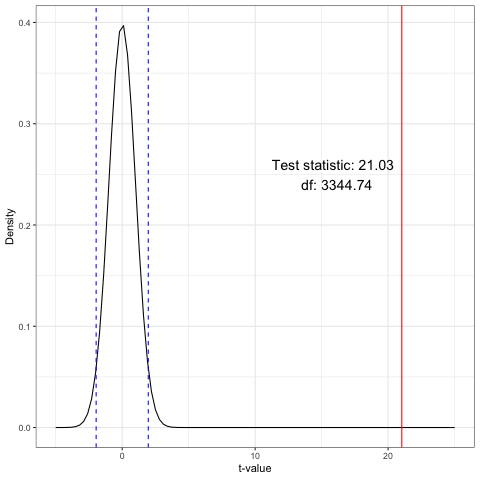
\includegraphics{../results/testplot.png}
\caption{}
\end{figure}

The above plot shows that our test statistic is far right of the
threshold and this is another evidence to reject the null hypothesis.

In conclusion, we reject the null hypothesis that there's no difference
between the average PM2.5 in Beijing and Shanghai.

\subsection{Beyond the project}\label{beyond-the-project}

There are some limitations in our analysis:

\begin{itemize}
\item
  The datasets we are using are time series data which means there
  exists dependencies in the datasets. For example, there could be a
  strong relationship between today's PM2.5 and tomorrow's PM2.5.
\item
  We have ignore many valuable features in the datasets due to time
  constraint. For example, we could include humidity and temperature of
  each day and create a regression model with PM2.5 value.
\end{itemize}

\subsection{Reference}\label{reference}

\begin{itemize}
\item
  \href{https://www.kaggle.com/uciml/pm25-data-for-five-chinese-cities}{PM2.5
  Data of Five Chinese Cities from Kaggle.com}
\item
  \href{https://en.wikipedia.org/wiki/Welch\%27s_t-test}{Welch's t-test
  from Wikipedia}
\end{itemize}


\end{document}
